\documentclass[11pt,a4paper]{article}
\usepackage[margin=0.88in,headheight=15pt,footskip=28pt]{geometry}
\usepackage[T1]{fontenc}
\usepackage{amsthm,amssymb}
\usepackage{lmodern}
\usepackage{microtype}
\usepackage{mathtools,bm}
\usepackage{booktabs,longtable,tabularx,array,multirow}
\usepackage{graphicx,caption,subcaption}
\usepackage{xcolor}
\usepackage{enumitem}
\usepackage{fancyhdr}
\usepackage{titlesec}
\usepackage{hyperref}
\usepackage[nameinlink,noabbrev]{cleveref}
\usepackage{float}
\usepackage{placeins}
\usepackage{listings}
\usepackage{setspace}
\usepackage{url}
\definecolor{ink}{HTML}{202A35}
\definecolor{accent}{HTML}{315B70}
\definecolor{muted}{HTML}{60717C}
\definecolor{pale}{HTML}{EDF2F4}
\hypersetup{colorlinks=true,linkcolor=accent,citecolor=accent,urlcolor=accent,pdfauthor={Devanik Debnath},pdftitle={Tame Moduli of Life}}
\setstretch{1.08}
\setlength{\parindent}{1.15em}
\setlength{\parskip}{3pt}
\setlist{nosep,leftmargin=1.5em}
\titleformat{\section}{\large\bfseries\color{ink}}{\thesection}{0.65em}{}
\titleformat{\subsection}{\normalsize\bfseries\color{accent}}{\thesubsection}{0.6em}{}
\titlespacing*{\section}{0pt}{1.5em}{0.55em}
\titlespacing*{\subsection}{0pt}{1.0em}{0.35em}
\pagestyle{fancy}
\fancyhf{}
\fancyhead[L]{\small\textsc{Tame moduli of life}}
\fancyhead[R]{\small\textsc{Research preprint \textbullet\ 31 October 2026}}
\fancyfoot[C]{\small\thepage}
\renewcommand{\headrulewidth}{0.35pt}
\renewcommand{\footrulewidth}{0pt}
\newtheorem{theorem}{Theorem}[section]
\newtheorem{proposition}[theorem]{Proposition}
\newtheorem{lemma}[theorem]{Lemma}
\newtheorem{corollary}[theorem]{Corollary}
\theoremstyle{definition}
\newtheorem{definition}[theorem]{Definition}
\newtheorem{assumption}[theorem]{Assumption}
\theoremstyle{remark}
\newtheorem{remark}[theorem]{Remark}
\newcommand{\R}{\mathbb{R}}
\newcommand{\N}{\mathbb{N}}
\newcommand{\ThetaSet}{\mathcal{P}}
\newcommand{\Life}{\mathcal{L}}
\newcommand{\Rep}{\mathcal{R}}
\newcommand{\Def}{\mathrm{Def}}
\newcommand{\Trop}{\operatorname{Trop}}
\newcommand{\supp}{\operatorname{supp}}
\newcommand{\poly}{\operatorname{poly}}
\newcommand{\doi}[1]{\href{https://doi.org/#1}{\texttt{doi:\detokenize{#1}}}}
\newcommand{\bzero}{b_0}
\newcommand{\format}{\mathcal{F}}
\newcommand{\degc}{D}
\newcommand{\eps}{\varepsilon}
\newcommand{\cR}{\mathcal{R}}
\newcommand{\cK}{\mathcal{K}}
\newcommand{\cS}{\mathcal{S}}
\newcommand{\cA}{\mathcal{A}}
\newcommand{\cW}{\mathcal{W}}
\newcommand{\cB}{\mathcal{B}}
\newcommand{\cT}{\mathcal{T}}
\newcommand{\cF}{\mathcal{F}}
\newcommand{\cD}{\mathcal{D}}
\newcommand{\cV}{\mathcal{V}}
\newcommand{\cE}{\mathcal{E}}
\newcommand{\cH}{\mathcal{H}}
\newcommand{\cM}{\mathcal{M}}
\newcommand{\cP}{\mathcal{P}}
\newcommand{\cL}{\mathcal{L}}
\newcommand{\cX}{\mathcal{X}}
\newcommand{\cY}{\mathcal{Y}}
\newcommand{\cZ}{\mathcal{Z}}
\newcommand{\cI}{\mathcal{I}}
\newcommand{\cQ}{\mathcal{Q}}
\newcommand{\cG}{\mathcal{G}}
\newcommand{\cC}{\mathcal{C}}
\newcommand{\cU}{\mathcal{U}}
\newcommand{\cO}{\mathcal{O}}
\newcommand{\cN}{\mathcal{N}}
\newcommand{\cYlife}{\mathcal{Y}_{\mathrm{life}}}
\newcommand{\cRcl}{\mathcal{R}_{\mathrm{cl}}}
\newcommand{\cWtr}{\mathcal{W}_{\mathrm{trop}}}
\newcommand{\cFwd}{\mathcal{F}_{\mathrm{wd}}}
\newcommand{\cEq}{\mathcal{E}_{\mathrm{eq}}}
\newcommand{\cAC}{\mathcal{A}_{\mathrm{C}}}
\newcommand{\cKtheta}{K_\theta}
\newcommand{\sgn}{\operatorname{sgn}}
\newcommand{\dist}{\operatorname{dist}}
\newcommand{\rank}{\operatorname{rank}}
\newcommand{\vol}{\operatorname{vol}}
\newcommand{\cl}{\operatorname{cl}}
\newcommand{\interior}{\operatorname{int}}
\newcommand{\bnd}{\partial}
\newcommand{\one}{\mathbf{1}}
\newcommand{\RR}{\mathbb{R}}

\begin{document}
\begin{titlepage}
\color{ink}
\vspace*{0.7cm}
{\large\textsc{Theoretical Research Series}}\hfill{\small PREPRINT \textbullet\ VERSION 1.0}
\vspace{1.4cm}
{\color{accent}\rule{\textwidth}{1.2pt}}
\vspace{0.55cm}
{\fontsize{27}{31}\selectfont\bfseries Tame Moduli of Life}\par
\vspace{0.28cm}
{\fontsize{16}{21}\selectfont\bfseries Sharp O-Minimal Finiteness for Repair-Closed Systems and Tropical Walls over the Landscape of Physical Laws}\par
\vspace{0.55cm}
{\color{accent}\rule{0.42\textwidth}{1.2pt}}
\vspace{0.75cm}
{\large\itshape Can a museum of every possible life form, in every possible universe, be finite?}\par
\vspace{1.25cm}
{\Large Devanik Debnath}\par
{\normalsize Department of Electronics and Communication Engineering\\National Institute of Technology Agartala, India}\par
{\small Public research profile: ECE '26 designation; no completed degree is asserted.}\par
\vspace{0.7cm}
\begin{minipage}{0.92\textwidth}
\small
\textbf{Abstract.} We formulate a conditional finiteness programme for families of repair-closed dynamical systems indexed by finite-dimensional parameters describing candidate physical laws. The central move is to encode a finite-dimensional admissibility predicate---positive catalytic production, a bounded state domain, and closure under a specified repair map---as a definable set in a fixed o-minimal expansion of the real field. O-minimality then implies finitely many connected components; when the chosen structure is sharply o-minimal and a format--degree filtration is available, the component and Betti complexity admit structure-dependent polynomial bounds in the degree at fixed format. We distinguish this theorem-shaped statement from the much stronger and unsupported claim that all logically conceivable universes or life forms form a finite set. A tropical companion construction identifies finite polyhedral candidate walls for leading-order balances in finite-support reaction systems. A worked semialgebraic toy family, reproducible numerical checks, and a symbolic-AI audit pipeline illustrate the architecture. All simulations are synthetic; they establish neither the existence of life beyond Earth nor an empirical biological phase boundary.
\end{minipage}
\vfill
\begin{tabularx}{\textwidth}{@{}lX@{}}
\textbf{Status} & Theoretical framework and synthetic mathematical demonstration; not peer reviewed and not submitted.\\
\textbf{Release date} & 31 October 2026\\
\textbf{Keywords} & o-minimality; sharp o-minimality; format--degree complexity; repair invariance; autocatalytic networks; tropical geometry; mathematical biology.\\
\textbf{Repository} & \url{https://github.com/Devanik21/The-Invention-Archive}
\end{tabularx}
\vspace{0.5cm}
\small\color{muted}Scope note: the term ``life'' is operationalized here as a model-relative conjunction of explicit mathematical predicates. No universal definition of life is proposed.
\end{titlepage}

\pagenumbering{roman}
\tableofcontents
\clearpage
\pagenumbering{arabic}

\section{The finite-museum question}
A useful mathematical version of the museum question is not whether there are finitely many individual organisms, species, chemical compositions, or possible universes. Even a single connected region of parameter space contains a continuum of parameter values. The more precise question is whether a specified family of candidate physical laws can partition into only finitely many connected classes with respect to an explicitly defined life-admissibility predicate. Such a result would give a finite number of ``rooms'' in a mathematical museum, not a finite number of specimens inside each room.

This distinction is decisive. A connected component of a subset of \(\R^p\) may contain uncountably many points. O-minimality excludes infinitely many disconnected definable pieces in a fixed finite-dimensional setting; it does not discretize a continuum, bound the number of states within a component, or prove that the set of all imaginable laws is small. A theorem about connected components is therefore a structural finiteness theorem, not a cosmic census.

The paper studies a controlled family \(\ThetaSet\subset\R^p\) of model parameters. A point \(\theta\in\ThetaSet\) specifies coefficients, boundary constraints, a finite reaction topology, and a repair rule from a predeclared template family. A predicate \(\Life(\theta)\) is true when the encoded system has a positive catalytic witness and a repair-closed admissible state set under the declared definition. The central result is conditional: if the parameter domain, maps, and predicate are definable in a fixed o-minimal structure, then \(\Life\) has finitely many connected components. If the structure also carries a sharp format--degree filtration and the encoded predicate has controlled complexity, the component count has a polynomial degree bound at fixed format.

The tropical part asks a complementary question. In a finite-support polynomial model, which leading-order balances can change as parameters vary? Tropical hypersurfaces provide piecewise-linear candidates for such transition walls. In this paper they are not identified automatically with exact biological phase boundaries. Their role is to expose a finite asymptotic skeleton that can be compared with the exact definable partition.

\section{Research posture and precise contribution}
The contribution is a formal bridge, not a claim to have solved the origin of life or classified all possible biochemistries. We make four separations throughout. First, established mathematical theorems about tame definable sets are not new biological discoveries. Second, a model-relative repair predicate is not a universal definition of life. Third, the toy model is a reproducible mathematical example, not observational evidence. Fourth, tropical walls are asymptotic candidates unless a lifting or non-degeneracy theorem connects them to the exact positive solution set.

The proposed architecture has three parts. The \emph{tame layer} encodes a finite-dimensional family of laws and repair constraints in an o-minimal structure. The \emph{network layer} supplies a stoichiometric autocatalytic witness and an explicit closure predicate for a finite repair policy. The \emph{tropical layer} replaces selected polynomial balance equations by finite piecewise-linear hypersurfaces in logarithmic coordinates. The layers share a parameter space but answer different questions: topological finiteness, mechanistic admissibility, and dominant-balance geometry.

The formal result we prove is an application theorem: a definable repair-admissibility predicate inherits o-minimal finiteness, and a sharply o-minimal complexity filtration yields a format-dependent polynomial bound in degree. The paper also gives a worked semialgebraic model with an exactly computable logarithmic binomial wall, a positive stoichiometric witness, and a repair map that contracts a quadratic damage proxy. These computations validate the declared identities for the toy model only.

\begin{table}[H]
\centering\small
\caption{Epistemic status of the paper's central statements.}
\begin{tabularx}{\textwidth}{@{}p{0.22\textwidth}p{0.35\textwidth}X@{}}
\toprule
Class & Statement & Status and boundary \\
\midrule
P1: mathematical identity & Definable subsets in an o-minimal structure have finite cell decompositions; sharp filtrations can bound topological complexity. & Established mathematics, conditional on the specified structure and complexity filtration.\\
P1: model identity & The toy repair map satisfies an exact quadratic contraction identity. & Proved algebraically and checked numerically in the released script.\\
P4: structural correspondence & Repair-admissibility can be represented as a definable predicate for a finite-dimensional model class. & A proposed formal bridge; applicability depends on the explicit encoding.\\
P4: asymptotic correspondence & Tropical walls summarize dominant balances of finite-support polynomial equations. & Established tropical methodology; exact phase-boundary interpretation requires additional hypotheses.\\
P5: research intuition & A finite tame moduli space may organize possible life-supporting law classes. & Motivating analogy only; not a claim about every universe.\\
\bottomrule
\end{tabularx}
\end{table}

\section{Prior work: tame landscapes, sharp complexity, and life-like networks}
O-minimality originated as a framework for controlling definable subsets of ordered fields. Its characteristic one-dimensional property is that each definable subset of the line is a finite union of points and intervals. Cell decomposition extends this control to higher dimensions and gives a robust notion of dimension and finite topological complexity. Standard references include van den Dries' treatment of tame topology and the model-theoretic literature on definable geometry \cite{vanDenDries1998,coste1999}.

The physical-landscape precedent is direct and important. Grimm's tameness conjecture proposes that the space of effective theories compatible with quantum gravity should be described by definable parameter spaces and tame geometric data \cite{grimm2022}. Grimm and Monnee analyze finiteness theorems and connected components in the type-IIB/F-theory flux landscape, including conjectures about geometric complexity and the obstruction to infinite tails of disconnected vacua near boundaries \cite{grimmMonnee2024}. Their work is a precedent for using tame geometry to constrain families of physical theories; it is not a proof about biological possibility.

Sharp o-minimality enriches bare finiteness with a complexity filtration. Binyamini, Novikov, and Zack introduce format and degree as two integers controlling definable-set complexity and prove sharp cell-decomposition and Betti-number bounds within the relevant axiomatic framework; related results establish effective counting bounds in restricted Pfaffian settings \cite{binyaminiNovikovZack2022,binyaminiNovikovZackWilkie2022}. Related work uses sharp o-minimality to quantify complexity in physical observables and quantum field theory; Grimm and van Vliet explicitly develop format--degree complexity as a physical measure in QFT \cite{grimmVanVliet2025}. We borrow this mathematical language, but do not assume every model of physical law is automatically represented in one of the currently established sharply o-minimal structures.

Autocatalytic sets and RAF theory supply a distinct biological precedent. Stoichiometric analyses identify five fundamental categories of minimal autocatalytic cores and use them to classify recurrent network motifs \cite{steel2013,blokhuis2020}. RAF theory formalizes reflexively autocatalytic, food-generated organization, while reviews emphasize that autocatalytic organization can be necessary for some life-like models without being sufficient for life itself \cite{hordijkSteel2017,hordijk2019}. A recent 2026 study further analyzes autocatalytic cores in diluted dynamical regimes and their stationary properties \cite{nandan2026}. We therefore use autocatalysis as one finite network-level witness, not as a complete definition of living systems.

Tropical and partial-tropical methods have been used to study chemical reaction networks and biochemical dynamics, including partial tropical equilibrations and model reduction \cite{desoeuvres2022,desoeuvres2024}. A 2026 article applies tropical geometry to bounded biochemical state spaces and redox configurations \cite{cobley2026}; a separate 2026 preprint explicitly connects tropical geometry with biochemical steady-state topology \cite{perry2026}. These works rule out any claim that tropical geometry in biochemistry is itself new. The narrower synthesis pursued here is the coupling of a tame parameter-space finiteness statement with a repair-closure predicate and a tropical wall decomposition for one fixed class of candidate laws.

\begin{table}[H]
\centering\small
\caption{Closest precedents and what this paper does not claim to reproduce.}
\begin{tabularx}{\textwidth}{@{}p{0.23\textwidth}p{0.38\textwidth}X@{}}
\toprule
Literature stream & Established result used & Delimitation in this paper \\
\midrule
Tame physical landscapes & Definability and finiteness of selected physical-theory loci. & No inference from string vacua to the biological domain without a new encoding.\\
Sharp o-minimality & Format--degree filtrations and topological/Betti complexity bounds. & No universal numerical bound is asserted without a concrete structure and ledger.\\
Autocatalytic cores & Finite structural classification of minimal stoichiometric motifs. & No extension of the five motif theorem to every chemistry or every law-set is claimed.\\
Tropical biochemical systems & Piecewise-linear dominant-balance analysis of finite reaction equations. & Tropical hypersurfaces are not assumed to equal exact viability boundaries.\\
O-minimal dynamical invariants & Model-theoretic study of invariants for discrete-time dynamics. & We restrict to finite-dimensional repair-closed predicates and identify the continuous-time obstacles.\\
\bottomrule
\end{tabularx}
\end{table}

\section{Mathematical preliminaries: definability and tame finiteness}
A structure \(\cS\) on the real field is a compatible collection of subsets of \(\R^n\) for all finite \(n\), closed under Boolean operations, Cartesian products, and coordinate projections, and containing the real algebraic sets. A set \(X\subset\R^n\) is \(\cS\)-definable if it belongs to this collection, with parameters allowed according to the chosen convention. A function is definable when its graph is definable. The closure under projections is essential: existential quantification over a definable witness is exactly projection of a definable set.

The structure is o-minimal when every definable subset of \(\R\) is a finite union of points and intervals. Cell decomposition then gives finite decompositions in higher dimensions. In particular, every definable set has finitely many connected components and finite Betti numbers. The number of components is not generally the number of points, and the finite decomposition does not make a continuum countable. These basic properties are the topological engine behind the conditional theorem below.

A sharply o-minimal structure refines this framework with a filtration \(\Omega_{F,D}\), where format \(F\) controls logical/geometric presentation complexity and degree \(D\) controls algebraic or analytic complexity within that format. The exact axioms and associated bounds depend on the chosen sharp structure. The useful schematic conclusion is that, at fixed format, topological complexity is bounded by a structure-dependent polynomial in degree. We write this generically as \(P_F(D)\) and do not assign coefficients or exponents without a concrete theorem and a concrete complexity audit.

The distinction between format and degree matters. Raising the ambient dimension, adding quantifier alternations, or introducing a new special function may increase format. Increasing polynomial degrees or the algebraic complexity of coefficients may increase degree. A claimed sharp bound is meaningful only when the formula's representation has been tracked under the allowed operations. A paper that labels a model ``tame'' but does not show that the maps and predicates lie in the chosen structure has not earned a finiteness certificate.

\begin{definition}[Admissible parameter family]
A finite-dimensional model family consists of a definable parameter domain \(\ThetaSet\subset\R^p\), a definable state-domain family \(K\subset\ThetaSet\times\R^n\), a definable vector field \(f:\ThetaSet\times\R^n\to\R^n\), a finite or definably parameterized family of repair maps \(R\), a definable damage functional \(V\), and a definable catalytic-witness predicate \(A(\theta,x)\).
\end{definition}

\begin{definition}[Repair closure]
For a fixed repair policy \(r\), the state set \(K_\theta\) is repair-closed when \(R_{\theta,r}(K_\theta)\subseteq K_\theta\). It is damage-nonincreasing when \(V_\theta(R_{\theta,r}(x))\leq V_\theta(x)\) for all \(x\in K_\theta\). In this paper a repair-closed admissible system is one satisfying both conditions for the declared policy and domain.
\end{definition}

\section{Operational life predicate and finite reaction witnesses}
A universal definition of life is intentionally avoided. Instead, we define a model-relative admissibility predicate. This is not a philosophical claim that all life must autocatalyze in the same way, nor does it settle whether nonchemical substrates are living. It provides a precise predicate against which a theorem can be stated and falsified.

Let a finite reaction network have \(n\) species and \(m\) reactions. Its stoichiometric matrix is \(S\in\R^{n\times m}\). A positive production witness is a flux vector \(v\in\R^m_{\geq0}\) satisfying \(Sv\gg0\) on the designated catalytic species. In a parameterized network, entries of \(S(\theta)\) and constraints on \(v\) must be definable. This stoichiometric criterion is a useful autocatalytic witness, but it is weaker than dynamical persistence, hereditary reproduction, open-ended evolution, or a complete theory of life.

The finite reaction list is important. If a network topology changes with \(\theta\), it must do so through a finite collection of definable cases, or through a finite-dimensional encoding that remains in the chosen structure. Infinite discrete switching encoded as an unrestricted subset of the real line is incompatible with o-minimality. The present framework therefore allows a finite menu of network topologies and a finite or definably parameterized repair-policy family. It does not allow arbitrary combinatorial objects to enter without a representation.

We use a state set \(K_\theta\) to encode physical admissibility, including positivity, resource bounds, and any conserved quantities explicitly included in the model. Repair is a map acting on the state, not a metaphor. Damage is a nonnegative functional chosen for the specific model. A decrease in this functional certifies only the stated mathematical contraction; it does not imply thermodynamic reversibility, absence of mutation, or biological rejuvenation.

\begin{definition}[Repair-admissible life region]
Let \(J\) be a finite repair-policy index set. Define
\[
\Life=\left\{\theta\in\ThetaSet:\ \exists j\in J\ \exists x\in K_\theta\cap\R^n_{>0}\ \exists v\in\R^m_{\geq0}:
\begin{array}{l}
f(\theta,x)=0,\quad S(\theta)v\gg0,\\
R_{\theta,j}(K_\theta)\subseteq K_\theta,\\
V_\theta(R_{\theta,j}(y))\leq V_\theta(y)\quad\forall y\in K_\theta
\end{array}\right\}.
\]
The quantifiers and inclusion are interpreted in the fixed definable model language. If policy parameters are continuous, their quantified domain must also be definable and finite-dimensional.
\end{definition}

\section{Why the predicate is definable}
The formula above is deliberately built from operations preserved by definability. The equilibrium equation is the zero set of a definable function. Positivity and resource constraints are definable inequalities. The stoichiometric witness is an existential quantifier over a finite-dimensional nonnegative orthant. A repair inclusion can be written as a first-order condition: for every state \(y\), if \((\theta,y)\in K\), then \((\theta,R_{\theta,j}(y))\in K\). The damage inequality is another universally quantified definable relation.

The existential quantifiers over \(x\), \(v\), and finite policy index \(j\) correspond to projections and finite unions. Universal quantification is expressible through complement and projection. Thus, when each primitive graph and domain is definable, the entire predicate is definable. This is the crucial transfer step. It is not enough that the differential equations look smooth or physically reasonable; their graphs and the logical conditions used to characterize admissibility must belong to the same structure.

A subtlety concerns continuous-time trajectories. The condition \(f(\theta,x)=0\) is a pointwise equilibrium condition and is algebraic or definable under standard assumptions. A statement such as ``every solution remains in \(K_\theta\) for all real times'' introduces the solution map of an ODE. That map need not be definable in a chosen structure merely because the vector field is definable. To include global trajectory claims, one must prove definability of the relevant flow on the domain and time interval, or replace the claim with a valid invariant-set certificate such as a definable Lyapunov or barrier condition. This paper uses the latter style in the worked model.

The repair policy is also restricted. An arbitrary operator on an infinite-dimensional function space is not covered by a finite-dimensional definability argument. A parameterized family of polynomial maps on a compact semialgebraic state set is covered. A finite list of policies is covered by finite disjunction. This restriction is not an inconvenience to hide; it is the hypothesis that makes the theorem true.

\begin{proposition}[Definability transfer]
Suppose \(\ThetaSet\), \(K\), the graph of \(f\), the stoichiometric data \(S\), the repair maps \(R_j\), and the damage function \(V\) are definable in an o-minimal structure \(\cS\). Suppose the policy family is finite and all state, flux, and repair conditions above are expressible using first-order quantification over definable sets. Then \(\Life\) is \(\cS\)-definable.
\end{proposition}
\begin{proof}
Each primitive relation is definable by assumption. Conjunctions and implications are Boolean combinations. The condition that a repair map sends every admissible state into the admissible domain is a universally quantified definable relation; universal quantification is obtained from complement and projection. The witness conditions on \(x\) and \(v\) are existential projections. A finite policy union is definable by closure under finite unions. Repeated use of closure under Boolean operations and coordinate projection therefore yields a definable subset of \(\ThetaSet\), which is exactly \(\Life\).
\end{proof}

\section{Conditional finiteness theorem}
The theorem is simple by design. The scientific work is shifted into the encoding audit: proving that a candidate family of laws and its repair/admissibility relations are genuinely definable in a fixed o-minimal structure. Once this is done, topological finiteness follows from established model theory. This is a powerful conditional theorem, but it is not a theorem about arbitrary possible universes.

\begin{theorem}[Finite tame repair landscape]
Let \(\cS\) be an o-minimal expansion of the real field. Let \(\ThetaSet\subset\R^p\) be definable, and let \(\Life\subseteq\ThetaSet\) be the repair-admissible life region of a finite-dimensional model family as defined above. If the primitive model data are \(\cS\)-definable, then \(\Life\) has finitely many connected components. Consequently, the admissible parameter landscape admits a finite partition into connected life-compatible regions and their complement.
\end{theorem}
\begin{proof}
By the definability-transfer proposition, \(\Life\) is \(\cS\)-definable. O-minimal cell decomposition partitions every definable subset of \(\R^p\) into finitely many cells. Each cell is connected, and a finite union of connected cells has at most finitely many connected components. The complement \(\ThetaSet\setminus\Life\) is also definable, so it too has finitely many connected components. No assertion is made that either region is finite as a set of points.
\end{proof}

\begin{corollary}[Uniformity for definable families]
If \(E\subseteq\Lambda\times\ThetaSet\) is definable in an o-minimal structure, then the number of connected components of each fibre \(E_\lambda\) is uniformly bounded as \(\lambda\) varies over \(\Lambda\).
\end{corollary}
\begin{proof}
This is the uniform finiteness property for definable families: cell decomposition compatible with the family gives a finite partition of the parameter space over which fibre topology is controlled. The bound depends on the fixed definable family, not on an unrestricted universe index.
\end{proof}

\begin{remark}
The finiteness theorem counts components in a fixed finite-dimensional parameterization. It does not say that a connected component contains finitely many law parameter values, nor that the number of components is invariant under enlarging the model class. A new physical degree of freedom, a new reaction topology, or a non-definable function may change the structure and invalidate the certificate.
\end{remark}

\section{Sharp complexity: format--degree bookkeeping}
Bare o-minimality is existential: it certifies that the number of components is finite, but it does not generally provide a usable numerical upper bound. Sharp o-minimality is relevant because it supplements the structure with a two-parameter complexity filtration. For a formula defining \(\Life\), let \((F_\Life,D_\Life)\) be a valid format--degree pair in the chosen sharp structure. Under the applicable sharp component or Betti bound, one obtains
\[
 b_0(\Life)\leq P_{F_\Life}(D_\Life),
\]
where \(P_F\) is the polynomial associated with format \(F\) by that structure's axioms or theorem. The expression is schematic until the structure and the exact complexity calculus have been fixed.

We propose a \emph{format--degree ledger} as an auditable object. Each primitive constraint is assigned a format and degree. Each operation---conjunction, disjunction, complement, projection, composition, finite union, and substitution---is recorded with the corresponding complexity propagation rule. The final life predicate inherits a bound only if every step is covered by a valid rule in the chosen structure. A hidden use of unrestricted sine, a non-definable solution map, or a quantified object outside the finite-dimensional domain breaks the chain.

This ledger also clarifies what a model-building AI should do. It must not merely suggest that a system is ``probably tame.'' It should return a symbolic representation of each primitive map, the structure in which it is definable, the operations used to assemble the predicate, and a degree/format propagation trace. A human reviewer must check the mathematical correctness of that trace. The output is a proof assistant for the encoding process, not an oracle that certifies arbitrary physics.

\begin{table}[H]
\centering\small
\caption{A proposed format--degree ledger for one finite model class. The symbols are placeholders until a concrete sharp structure is selected.}
\begin{tabularx}{\textwidth}{@{}p{0.25\textwidth}p{0.26\textwidth}p{0.18\textwidth}X@{}}
\toprule
Object & Definable representation & Ledger entry & Audit obligation \\
\midrule
Parameter domain & finite polynomial inequalities & \((F_\Theta,D_\Theta)\) & Verify domain and parameter bounds.\\
State constraints & positivity, conservation, compact bounds & \((F_K,D_K)\) & Confirm no hidden infinite-dimensional variables.\\
Dynamics & finite polynomial/rational vector field & \((F_f,D_f)\) & Denominator non-vanishing and domain.\\
Network witness & \(S(\theta)v\gg0,\ v\geq0\) & \((F_S,D_S)\) & Fixed finite species/reaction indexing.\\
Repair closure & quantified graph inclusion and damage inequality & \((F_R,D_R)\) & Track quantifiers and composition.\\
Final predicate & first-order combination and projection & \((F_\Life,D_\Life)\) & Apply the exact sharp propagation rules.\\
\bottomrule
\end{tabularx}
\end{table}

\section{Tropical walls from finite-support balances}
Let a polynomial balance equation have finite support
\[
P(x)=\sum_{\alpha\in A} c_\alpha x^\alpha,
\qquad A\subset\N^n\text{ finite}.
\]
Under a valuation or asymptotic scaling of coefficients and variables, write \(x_i=\exp(z_i/\eps)\) and coefficient valuations \(\nu(c_\alpha)\). The associated tropical polynomial is the piecewise-linear function
\[
\operatorname{trop}(P)(z)=\min_{\alpha\in A}\{\nu(c_\alpha)+\langle\alpha,z\rangle\}.
\]
Its tropical hypersurface consists of points where the minimum is attained at least twice. Because \(A\) is finite, the hypersurface is a finite union of polyhedral cells. Intersections of finitely many such hypersurfaces form a finite polyhedral complex after an appropriate common refinement.

This construction identifies candidate dominant-balance walls. It does not imply that every point on the tropical hypersurface lifts to a positive real solution of the original biochemical equations. Signs matter; positive real feasibility may require signed tropical geometry, initial-form conditions, and non-degeneracy assumptions. Even when a tropical point lifts to a steady state, that steady state need not be stable, repair-closed, or biologically meaningful.

For the toy binomial \(ab-c=0\) with positive parameters, the logarithmic equation is especially simple:
\[
\log a+\log b-\log c=0.
\]
The tropical wall in log-parameter coordinates is exactly affine because there are only two monomials. In more general sums, tropicalization gives a piecewise-linear skeleton. The distinction between exact binomial equality and asymptotic tropical approximation is preserved in the figure captions and numerical outputs.

\begin{figure}[H]\centering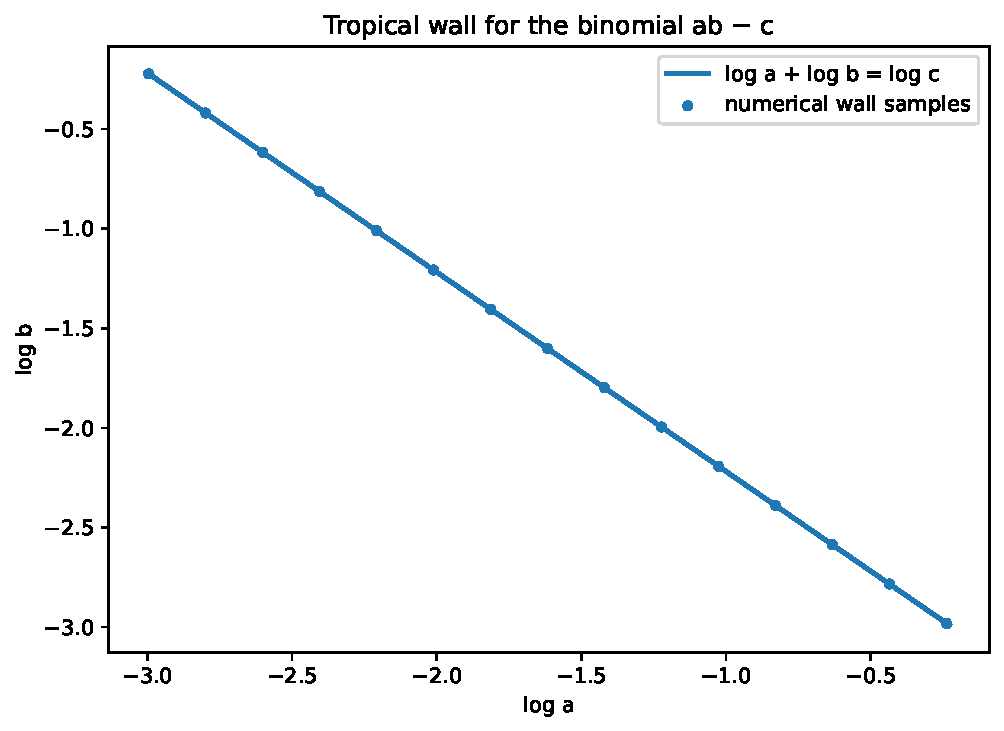
\includegraphics[width=0.72\textwidth]{figures/fig04_tropical_wall.pdf}\caption{The exact logarithmic wall of the synthetic binomial balance \(ab-c=0\). The residual is computed directly from the sampled positive points; the plot is a numerical check of an exact algebraic identity.}\label{fig:trop}\end{figure}

\section{The tame--tropical interface}
The tame and tropical constructions are complementary rather than interchangeable. The tame predicate labels the exact admissible region in a chosen finite-dimensional model class. Tropical walls summarize the leading-order combinatorics of selected polynomial equations. The exact boundary \(\bnd\Life\) is definable whenever \(\Life\) is definable, because closure and complement preserve definability. The tropical wall set is finite polyhedral when the underlying support and valuation data are finite. Neither set is automatically equal to the other.

A practical interface can be organized in three steps. First, construct the exact definable formula and compute or bound its format--degree complexity. Second, tropicalize only the balance equations for which a meaningful coefficient valuation or scale separation is available. Third, compare the projected tropical cells with the exact life/non-life partition using certified inequalities, numerical continuation, or a theorem on lifting. The comparison should identify false-positive tropical walls, missing positive branches, and regions where the asymptotic approximation is poor.

The wall arrangement may stratify the parameter domain into finitely many candidate regimes. The exact tame partition also has finitely many cells. A common refinement can therefore provide a finite combinatorial atlas for a given model class. This is the strongest defensible reading of the ``museum floor plan'': a finite atlas of regimes, each of which may contain a continuum of model parameters and states.

\begin{figure}[H]\centering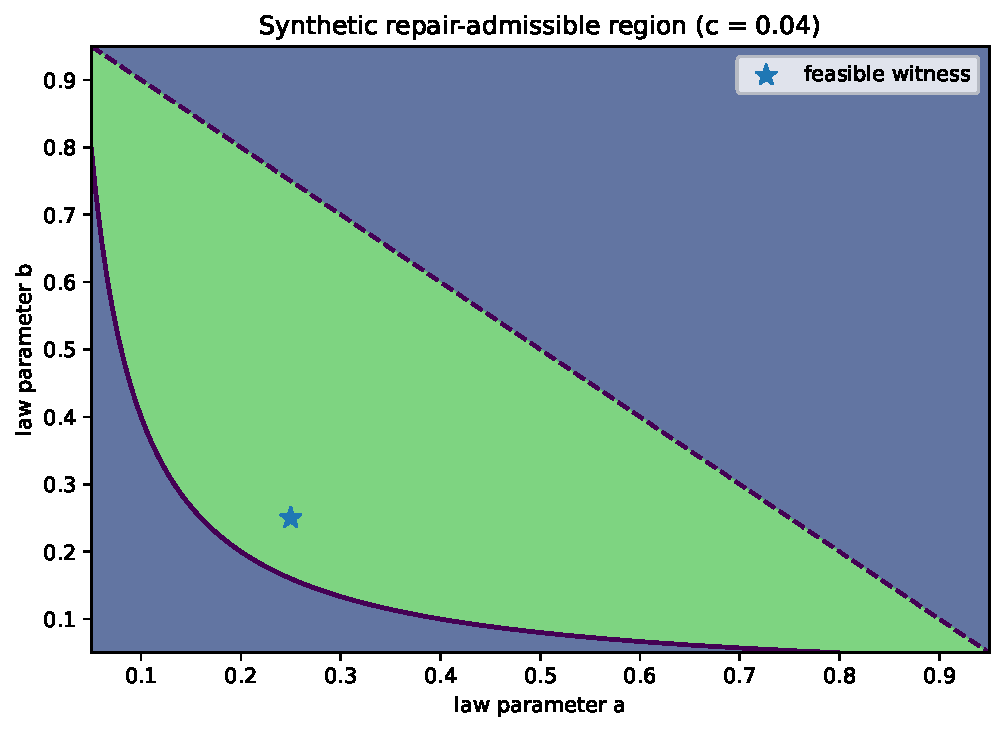
\includegraphics[width=0.83\textwidth]{figures/fig01_life_region.pdf}\caption{A two-parameter slice of the toy repair-admissible region at fixed \(c=0.04\). The exact inequalities are \(a,b\geq0.05\), \(a+b\leq1\), and \(ab\geq c\). The shaded set is one connected region on the displayed grid; the grid count is not used as proof of the theorem.}\label{fig:life}\end{figure}

\section{Worked model: a finite repair-closed family}
We instantiate the architecture with a deliberately simple family indexed by \(\theta=(a,b,c)\), where \(a\) and \(b\) are two positive catalytic-capacity parameters and \(c\) is a damage burden. All values are dimensionless. The parameter box is \(a,b\in[0.05,0.95]\), \(c\in[0.005,0.20]\). The admissibility inequalities are
\[
 a+b\leq1,\qquad ab\geq c.
\]
The first is a resource budget and the second is a repair-capacity margin. The model is semialgebraic. For fixed \(c\), the slice is a closed semialgebraic subset of a compact square.

The catalytic network has two species, \(A\) and \(B\), with reactions \(A+B\to2A+B\) and \(A+B\to A+2B\). Its stoichiometric matrix is \(S=I_2\). The flux \(v=(1,1)^\top\) gives \(Sv=(1,1)^\top\gg0\), so the positive-production witness holds identically. This is a minimal synthetic mutual-amplification motif used only to supply the formal witness. It is not asserted to represent a real prebiotic chemistry.

The state domain is \(K=[0,1]^2\). For a target state \(\theta_*=(a,b)\), let the repair map be the convex interpolation
\[
R_\lambda(x;\theta_*)=(1-\lambda)x+\lambda\theta_*,\qquad \lambda\in[0,1].
\]
Since the square is convex, \(R_\lambda(K)\subseteq K\). With quadratic damage \(V(x;\theta_*)=\|x-\theta_*\|_2^2\), one has \(V(R_\lambda(x);\theta_*)=(1-\lambda)^2V(x;\theta_*)\leq V(x;\theta_*)\). Hence the state domain is repair-closed and damage-nonincreasing for every allowed \(\lambda\). The global life predicate for this model reduces to the two inequalities above plus the positive catalytic witness.

\begin{figure}[H]\centering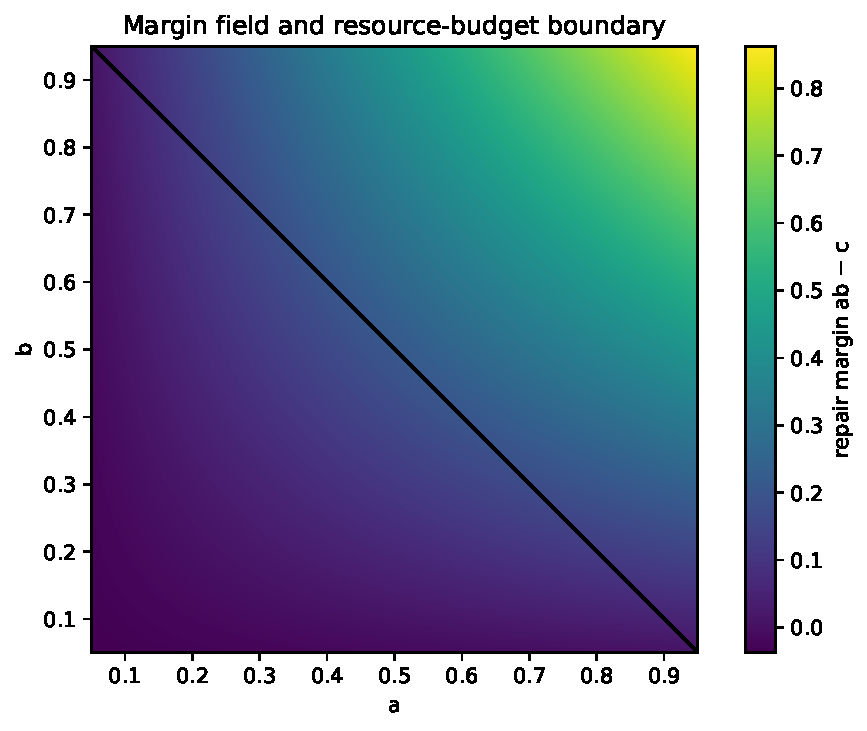
\includegraphics[width=0.76\textwidth]{figures/fig02_margin_field.pdf}\caption{The synthetic repair margin \(ab-c\) on the \((a,b)\) slice. Positive values satisfy the capacity threshold; the additional resource budget \(a+b\leq1\) restricts the admissible domain.}\label{fig:margin}\end{figure}

\section{Analytical geometry of the toy life region}
For fixed \(c\in(0,1/4)\), the product boundary \(ab=c\) is a decreasing hyperbola in the positive quadrant. The budget boundary \(a+b=1\) is a line. The two intersect when \(a(1-a)=c\), giving
\[
a_\pm=\frac{1\pm\sqrt{1-4c}}{2},\qquad b_\pm=1-a_\pm.
\]
For \(c=0.04\), the roots are approximately \(0.041742\) and \(0.958258\). The displayed state-domain floor of \(0.05\) clips the lower endpoint of the feasible slice, but a feasible point such as \((0.25,0.25)\) satisfies both constraints. The mathematical example therefore has a nonempty admissible region.

The grid experiment uses an \(801\times801\) mesh across \([0.05,0.95]^2\). Eight-neighbour connected-component labeling reports one connected component on that discretization. The estimated area is approximately \(0.3323\) in the displayed parameter coordinates. These numbers depend on the grid convention and are reported only as reproducibility outputs; the connectedness statement for this simple slice can be established analytically from the monotone boundary and convex budget region, not from grid labeling. We do not confuse a rasterized count with a topological proof.

The boundary \(ab=c\) is a binomial hypersurface, so its logarithmic representation is exact. The budget boundary is also algebraic, but its tropicalization is interpreted with the signed coefficient data and an explicit valuation convention. The numerical script plots the exact product wall, evaluates the logarithmic residual, and separately records the budget constraint. Figure \ref{fig:trop} is therefore not presented as a full tropicalization of the two-inequality life predicate; it shows the binomial capacity wall only.

\begin{table}[H]
\centering\small
\caption{Toy-model parameters and one verified feasible witness.}
\begin{tabularx}{\textwidth}{@{}p{0.22\textwidth}p{0.20\textwidth}p{0.20\textwidth}X@{}}
\toprule
Quantity & Symbol & Value & Role \\
\midrule
Catalytic capacity A & \(a\) & 0.25 (witness) & Positive parameter in the product-capacity criterion.\\
Catalytic capacity B & \(b\) & 0.25 (witness) & Positive parameter in the product-capacity criterion.\\
Damage burden & \(c\) & 0.04 & Threshold requiring \(ab\geq c\).\\
Resource budget & -- & \(a+b\leq1\) & Restricts the admissible parameter region.\\
Repair fraction & \(\lambda\) & \([0,1]\) & Convex interpolation coefficient.\\
State domain & \(K\) & \([0,1]^2\) & Compact convex invariant set.\\
\bottomrule
\end{tabularx}
\end{table}

\section{Numerical verification and reproducibility}
The released verifier implements the toy inequalities, the stoichiometric witness, the repair map, the quadratic damage function, the tropical logarithmic residual, and a one-dimensional degree/component illustration. Randomness is not used in the model calculations; a fixed seed is recorded for consistency if the script is extended. The script uses NumPy for arrays, SciPy for connected-component labeling, Matplotlib for vector and raster plots, and NetworkX for graph diagrams. The exact Python and package versions are written to the result report.

The repair contraction is checked at 21 values of \(\lambda\in[0,1]\). For each value, the verifier compares the directly evaluated damage after repair with the exact identity \((1-\lambda)^2V(x)\), and asserts non-increase. The tropical wall residual is evaluated at positive samples satisfying \(b=c/a\); the maximum floating-point residual is approximately \(4.44\times10^{-16}\), consistent with round-off. A feasible witness is checked directly, and the positive production witness is evaluated using the declared stoichiometric matrix.

The degree demonstration uses polynomials with evenly spaced simple real roots and records the number of connected intervals on which the polynomial is nonnegative. It illustrates degree-sensitive behaviour in a one-dimensional algebraic family and is not a universal theorem about arbitrary definable sets. A grid-resolution table records approximate area and component counts for four resolutions. The plots and CSV files are generated in the release directory, so the PDF's data-bearing figures can be rebuilt from the released source.

\begin{figure}[H]\centering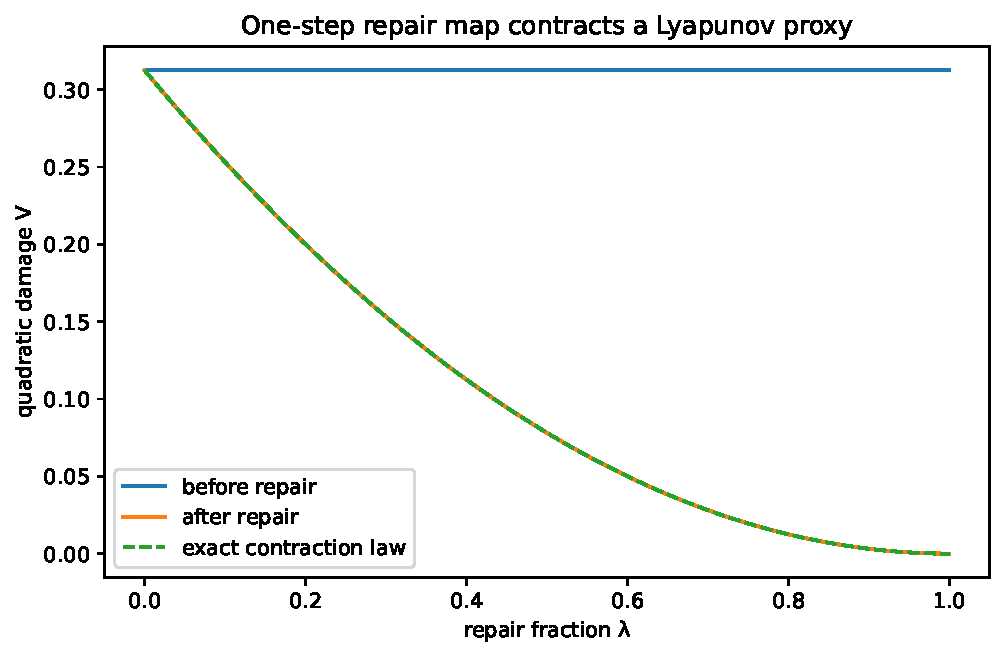
\includegraphics[width=0.72\textwidth]{figures/fig03_repair_contraction.pdf}\caption{Quadratic damage before and after repair for a fixed state and target. The exact contraction curve is shown beside direct evaluations of the map. Synthetic identity check; no biological repair rate is inferred.}\label{fig:repair}\end{figure}

\begin{figure}[H]\centering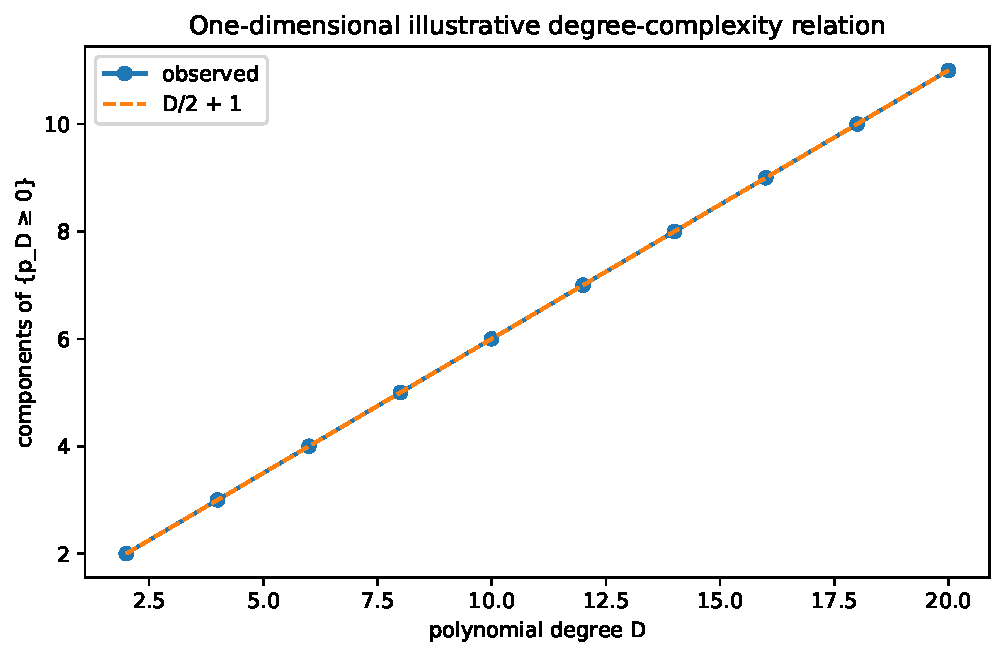
\includegraphics[width=0.72\textwidth]{figures/fig05_degree_components.pdf}\caption{Connected components of one-dimensional polynomial sign sets as degree increases. The observed count matches the constructed root pattern, providing a transparent example of degree-sensitive topological complexity.}\label{fig:degree}\end{figure}

\section{Network representation and repair-state graph}
A network diagram is useful here only when its semantics are explicit. Figure \ref{fig:network} shows the two-species autocatalytic toy motif used for the stoichiometric witness. The loops represent positive net production of each species under the chosen reaction channels; dashed cross-links indicate that both species appear among the co-reactants. The matrix identity \(S=I_2\) and flux \(v=(1,1)\) are the numerical objects actually checked.

Figure \ref{fig:stategraph} represents a discretized state-transition graph under an illustrative repair update. Its nodes are a coarse grid over a two-dimensional state square and its directed edges show the chosen coarse update. The graph is not the exact continuum dynamics and it is not evidence of an observed biological attractor. Its purpose is to distinguish the finite graph used for visualization from the continuous definable state domain used in the theorem.

This distinction will matter in applications to real reaction networks. A reaction graph can be finite even when its dynamics has a continuum of trajectories. Conversely, a finite-state abstraction can hide non-definable features or singularities if the abstraction is not faithful. A defensible workflow should retain the original stoichiometric matrix, kinetic equations, state constraints, and a proof that the abstraction preserves the predicate of interest.

\begin{figure}[H]\centering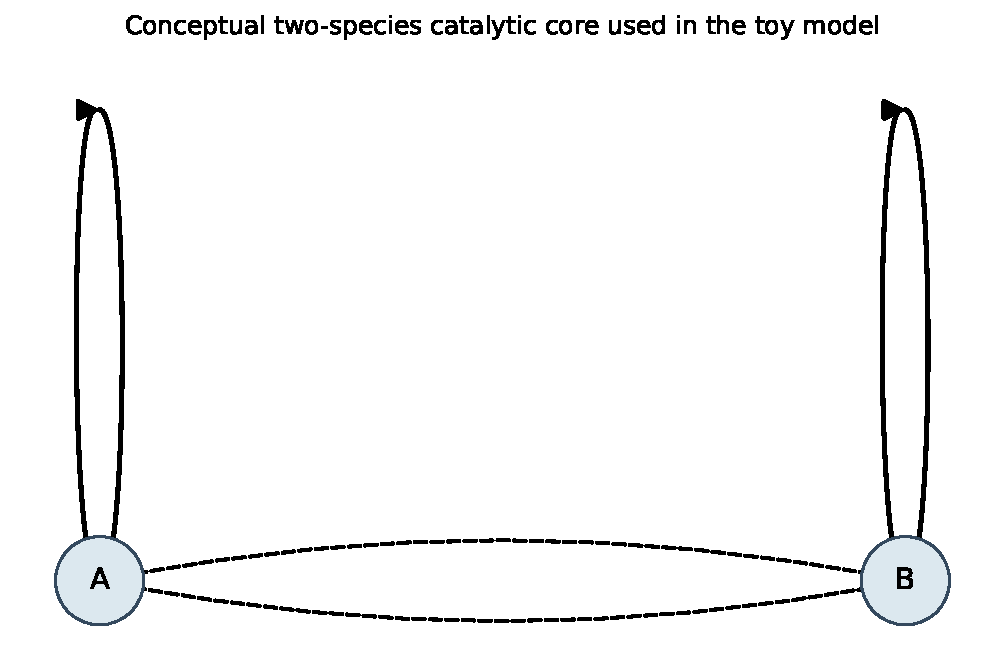
\includegraphics[width=0.72\textwidth]{figures/fig07_autocatalytic_graph.pdf}\caption{Directed network representation of the synthetic two-species autocatalytic core. Its positive stoichiometric production witness is \(Sv=(1,1)^\top\). The graphic is conceptual and model-specific.}\label{fig:network}\end{figure}

\begin{figure}[H]\centering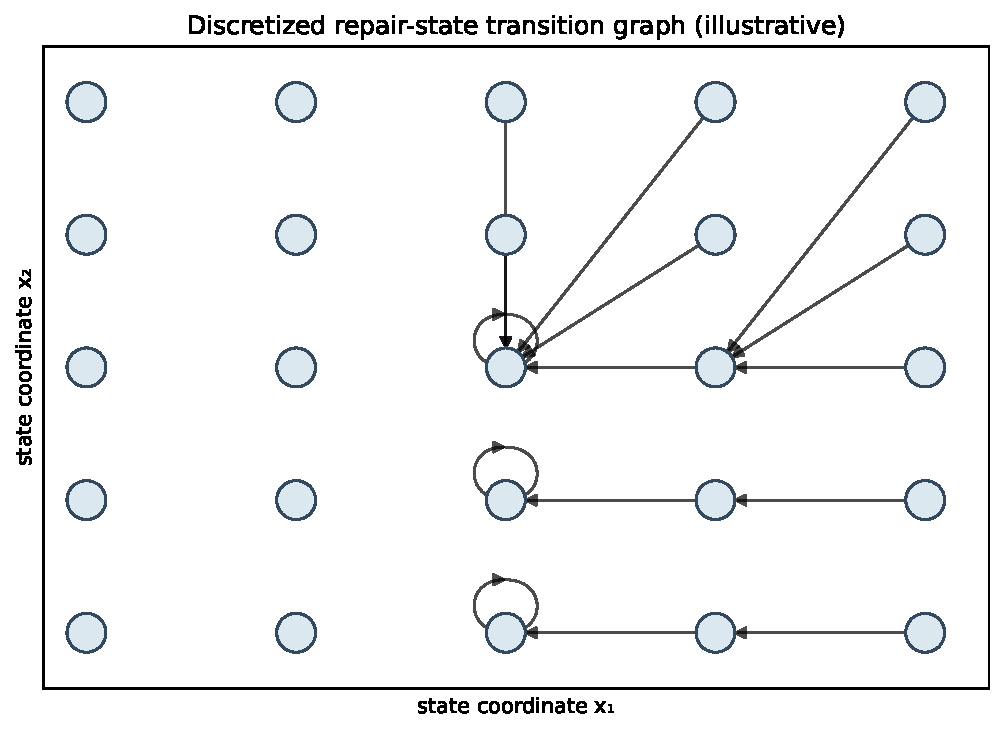
\includegraphics[width=0.72\textwidth]{figures/fig08_repair_state_graph.pdf}\caption{Discretized state-transition graph for an illustrative repair update. This finite graph is a visualization of a grid abstraction, not the state space or trajectory set used in the theorem.}\label{fig:stategraph}\end{figure}

\section{AI's role: symbolic model compilation and adversarial audit}
Artificial intelligence is useful in this programme only if it contributes a verifiable computation. We propose a constrained symbolic pipeline: ingest a finite mechanistic model specification; parse reactions, parameters, state constraints, and repair rules into a typed symbolic abstract syntax tree; propose candidate first-order predicates; produce a format--degree ledger for a named sharp structure; generate a tropical support table; and emit counterexample queries and a validation script. A separate proof checker or computer algebra system should validate algebraic identities and sign conditions. The AI component must not be allowed to certify statements by natural-language plausibility alone.

An AI model can help discover missing assumptions and propose alternative representations. For example, it may detect that an apparent ``repair'' map is not invariant on the stated domain, that a denominator can vanish, that a positive-flux witness fails at a boundary parameter, or that an unrestricted trigonometric term invalidates the claimed o-minimal setting. It can also propose adversarial values near the boundary of the life region, where a finite mesh is least reliable. These tasks are well suited to AI-assisted symbolic review because every proposed counterexample can be checked by an independent numerical or algebraic routine.

The nontrivial AI research question is whether such a system can reliably translate mechanistic model descriptions into formal predicates without silently changing their semantics. A valid benchmark would include positive cases, false-life cases, non-definable cases, invalid repair maps, missing witness species, and formula-complexity explosions. Metrics should include soundness of generated predicates, false-positive rate for claimed definability, proof-certificate completion rate, and complexity growth under projection and composition. The benchmark must not score fluent explanations as mathematical correctness.

\begin{figure}[H]\centering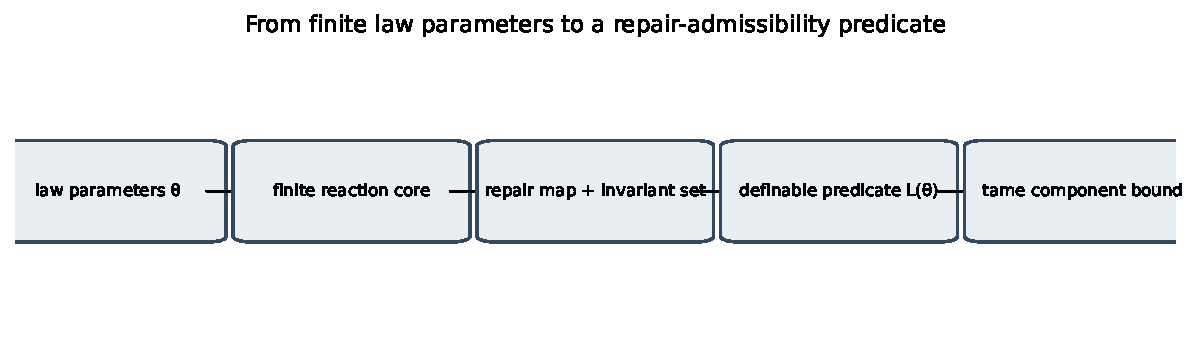
\includegraphics[width=0.9\textwidth]{figures/fig09_model_flow.pdf}\caption{The mathematical model pipeline: finite parameters and reaction topology are translated into an explicit repair-admissibility predicate before applying tame-geometric finiteness.}\label{fig:modelFlow}\end{figure}

\begin{figure}[H]\centering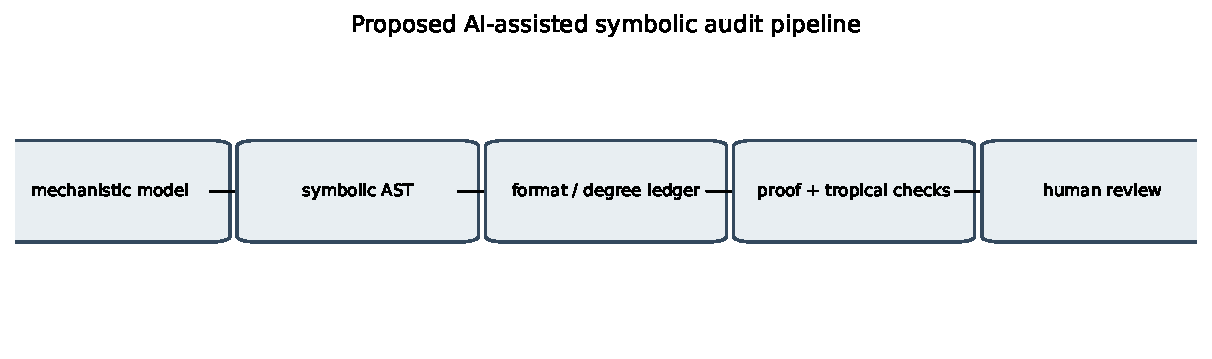
\includegraphics[width=0.9\textwidth]{figures/fig10_ai_audit_flow.pdf}\caption{Proposed AI-assisted symbolic audit. AI proposes and audits structured representations; formal checking and human review remain mandatory.}\label{fig:aiFlow}\end{figure}

\section{Falsification, negative controls, and failure criteria}
A useful theorem-shaped research programme needs failure criteria. The main mathematical claim fails for a proposed model family if the admissibility predicate cannot be shown definable in the chosen structure. Examples include unrestricted oscillatory functions with infinitely many zeros on a compact interval, arbitrary infinite discrete switching, non-definable coefficient encodings, or a continuous-time flow map for which definability has not been established. In these cases the correct output is not to force the model into an o-minimal framework; it is to change the model class, prove a stronger theorem in another framework, or abandon the finiteness claim.

The repair-closure claim fails if there exists a state \(x\in K_\theta\) for which the repair map exits \(K_\theta\), or if the declared damage functional increases when non-increase is required. A positive catalytic witness fails if no nonnegative flux satisfies the stipulated strict production inequalities. The tropical approximation fails as a phase-boundary proxy if the predicted wall has no corresponding positive real branch, if signed initial forms eliminate the lift, or if numerical continuation shows that the exact admissible boundary departs from the leading-order skeleton in the claimed regime.

Negative controls should include a model with no repair policy, a model with an intentionally non-invariant map, a reaction network whose stoichiometric matrix cannot produce every required species, and a parameter set whose only feasible point lies on a forbidden boundary. A particularly important control is a non-tame extension such as a function with an infinite oscillatory zero set. It should cause the definability audit to reject the o-minimal certificate, rather than trigger an invalid theorem application.

\begin{figure}[H]\centering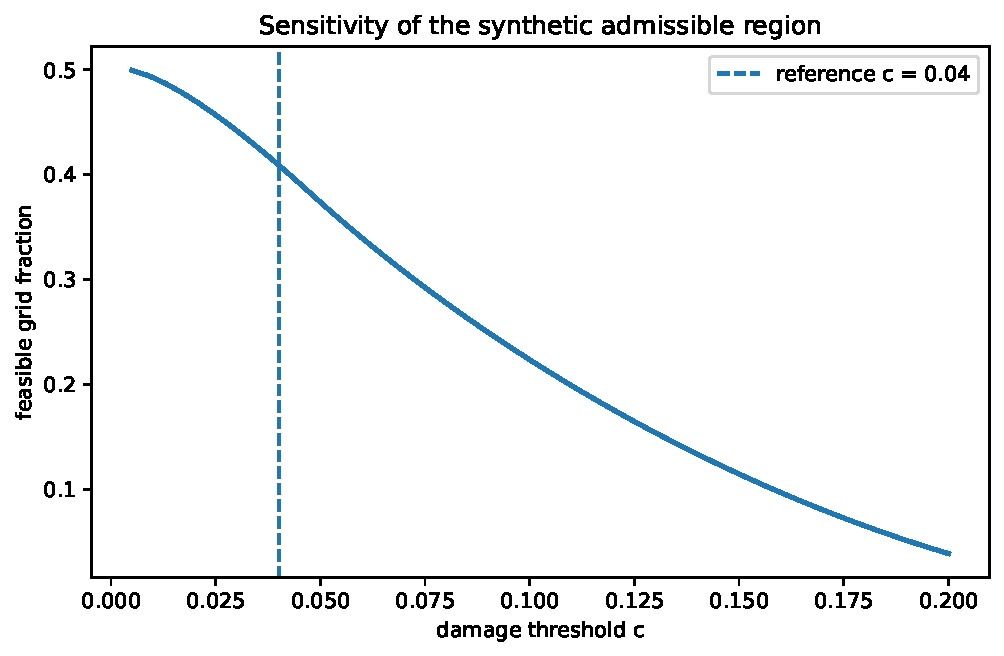
\includegraphics[width=0.74\textwidth]{figures/fig06_threshold_sensitivity.pdf}\caption{Feasible grid fraction as the synthetic damage threshold varies. This sensitivity analysis concerns one toy parameterization and has no biological calibration.}\label{fig:sensitivity}\end{figure}

\section{Sensitivity, approximation error, and robustness}
A finite connected-component theorem does not imply robust membership. A parameter point may sit arbitrarily close to the boundary of \(\Life\), so small coefficient perturbations can switch its label. To quantify robustness, define a model-specific signed margin such as \(m(\theta)=a b-c\) in the toy example. A strictly positive margin gives a quantitative buffer for that inequality, while the budget margin \(1-a-b\) controls the second constraint. The minimum of the two margins can be used as a simple robustness score only after scaling and units have been declared.

The numerical grid is an approximation layer. Its resolution controls boundary localization and area estimation. In a higher-dimensional model, uniform grids become computationally infeasible, and adaptive subdivision or certified interval methods are preferable. None of these algorithms replaces the topological theorem. Conversely, a theorem does not return the actual boundary, the number of components in a specific instance, or a useful experimental design. The theorem and the computational exploration solve different tasks.

The verifier checks area estimates at 101, 201, 401, and 801 grid points per axis. The estimated area approaches a stable value under refinement, but it remains a Riemann-sum approximation. Figure \ref{fig:convergence} shows this behavior. Figure \ref{fig:tropResidual} shows the absolute logarithmic residual on the exact binomial wall; it is a floating-point diagnostic rather than a proof of the identity. The analytical derivation in the text is the proof.

\begin{figure}[H]\centering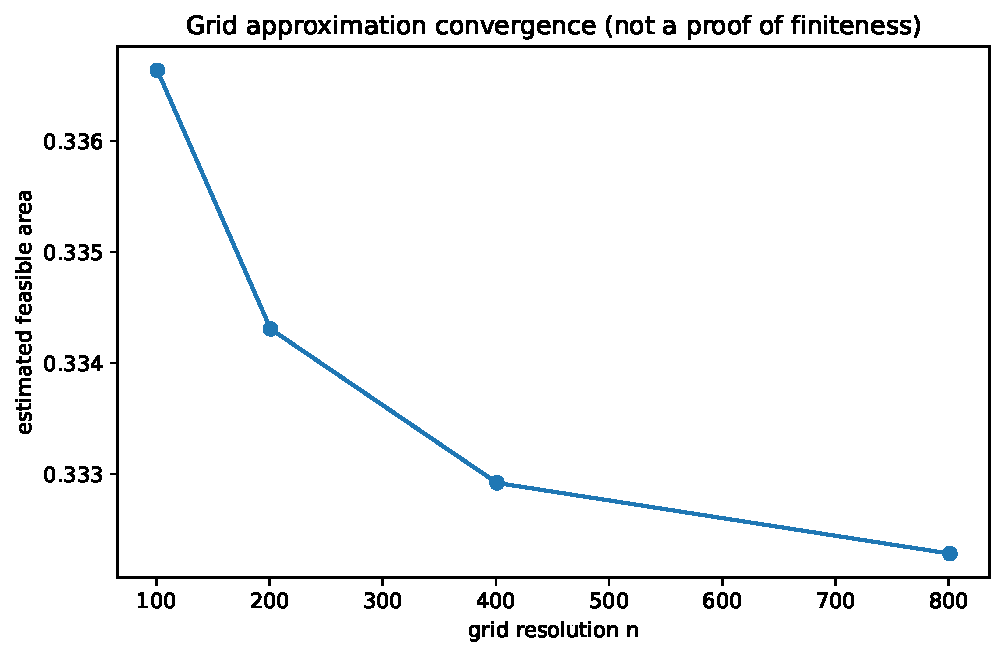
\includegraphics[width=0.72\textwidth]{figures/fig11_grid_convergence.pdf}\caption{Grid-resolution convergence of the estimated area of the toy life region. This is numerical approximation evidence, not a topological certificate.}\label{fig:convergence}\end{figure}

\begin{figure}[H]\centering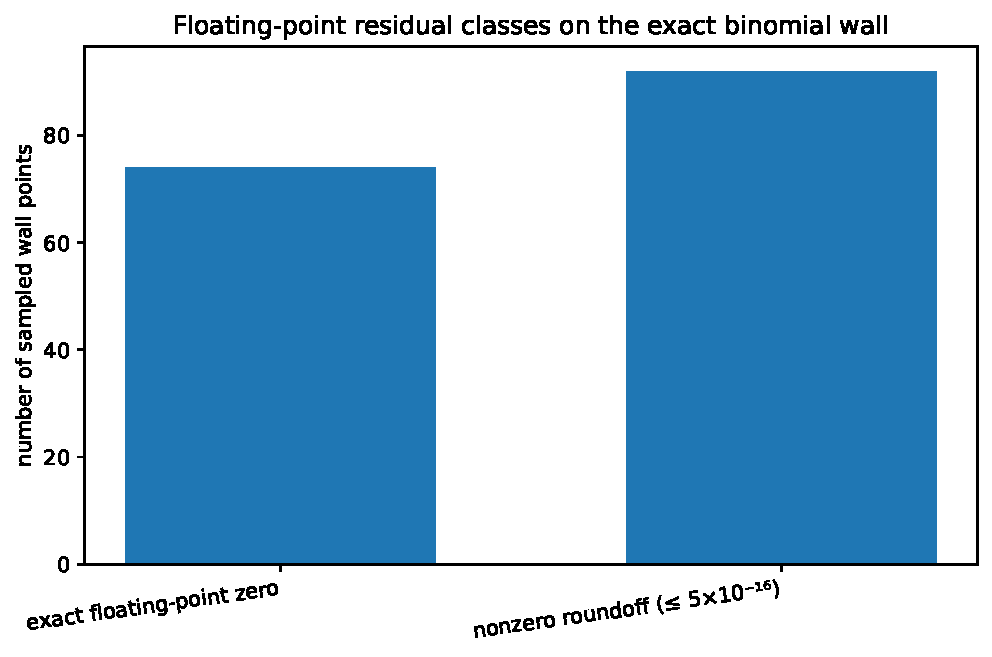
\includegraphics[width=0.72\textwidth]{figures/fig12_tropical_residual.pdf}\caption{Counts of sampled points with exactly zero floating-point residual and with a nonzero residual bounded by $5\times10^{-16}$ for the logarithmic binomial relation on $ab=c$. The exact identity follows algebraically; the counts only summarize roundoff in this implementation.}\label{fig:tropResidual}\end{figure}

\section{Landscape stratification as a finite atlas}
A finite tame atlas can be constructed by taking a cell decomposition compatible with the exact life region, its complement, and a finite collection of tropical candidate walls. Each cell carries labels: life-admissible or not, active repair policy, autocatalytic witness type, dominant-balance regime, and the associated format--degree metadata. A cell is a connected geometric piece, not a single universe. The atlas is useful because a model analyst can compare parameter regions without enumerating every parameter value.

The stratification can be refined when new mechanisms are added. For example, a different network topology may require a new finite disjunct in the predicate. A new repair policy may add a quantifier over a parameterized map. A new conservation law may add a definable equality. Each refinement changes the formula and hence the complexity ledger. The number of cells can grow substantially, even when it remains finite. The sharp bound is thus not a claim that the atlas is small in practice; it is a way to express a computable upper bound once the relevant format and degree are known.

The atlas also supports a clean separation of mathematical and physical uncertainty. Mathematical uncertainty concerns whether the chosen structure, filtration, and derivations are correct. Model uncertainty concerns whether the state variables and repair predicates represent the physical system adequately. Empirical uncertainty concerns the values of kinetic coefficients, the existence of the proposed reactions, and the stability of the measured system. A single geometric picture should not collapse these distinct uncertainties into one color or one number.


\section{Generalization beyond terrestrial biochemistry}
The parameterization need not describe carbon-based chemistry. It could encode a finite-dimensional model of catalytic reaction networks in a solvent, mineral-surface chemistry, a computational substrate, or a theoretical field system. What transfers is the formal architecture: a finite state description, a declared admissible domain, a repair or error-correction operation, a positive production or information-maintenance witness, and definable parameter dependence. The biological interpretation of each element must be re-established in the target substrate.

For abiotic systems, the phrase ``repair'' may mean error correction or restoration of a macroscopic invariant rather than biological healing. A network may display autocatalysis without reproduction, evolution, or life. A computational substrate may restore an internal codeword without metabolism. Therefore, substrate-agnostic language is permitted only when the predicate is explicitly renamed and its semantics are stated. Our use of ``life-admissible'' remains tied to the declared operational definition, not to the entire concept of life.

The main obstacle to extending the method across different physical laws is that the space of laws may be infinite-dimensional or involve unrestricted functions. A finite vector of coefficients does not capture every possible metric, field, or interaction. One route is to study finite-dimensional truncations or finite-dimensional moduli spaces of laws, then quantify how the result changes as the truncation dimension increases. Another is to find a different tame structure suited to the function class. Neither route justifies taking a limit over all possible laws without a uniform theorem.


\section{Relation to the string landscape and the meaning of finiteness}
The string-landscape analogy is methodological. In string theory, finiteness arguments apply to carefully specified moduli spaces, flux constraints, Hodge-theoretic data, and tadpole bounds. A result about a self-dual flux locus is not a result about every conceivable effective theory, still less about all possible universes. Our proposed life landscape is similarly restricted: it is a space of parameters and maps for which the model predicates are definable and the sharp complexity filtration is known.

The phrase ``finite museum'' is retained as an explanatory metaphor, but it needs a mathematical caption. It means finite connected components or finite cell count in a fixed definable parameter domain. It does not mean finitely many possible molecules, organisms, chemical networks, planets, or universes. One room may contain a continuum of parameter points and a continuum of trajectories. An atlas with finite cells can nevertheless be a useful finite classification of qualitative regimes.

A central open question is whether physically motivated classes of repair-closed systems can be shown to lie in a particularly useful sharply o-minimal structure, with an explicit degree ledger whose complexity depends in a controlled way on species count, reaction count, polynomial degree, and the number of repair-policy parameters. This is the route to a quantitative theorem that could be compared across model families. It is not solved here.


\section{Database and novelty audit}
The literature pass searched combinations of ``o-minimal'', ``o-minimality'', ``biology'', ``biochemical'', ``autocatalytic'', ``reaction networks'', ``life'', and ``systems biology'', alongside the established model-theory, mathematical-physics, RAF, and tropical-reaction-network literatures. The publicly visible MathSciNet pages retrieved in this session exposed Mathematical Subject Classification browse material for mathematical biology (including 92B and 92C) but did not expose a reproducible, record-level search result set for the exact cross-domain query. The public zbMATH material retrieved exposed the MSC2020 taxonomy, not a complete indexed-result export for the same query. Consequently, this audit does not certify that MathSciNet or zbMATH contains no prior application.

The current literature does include directly adjacent topics that rule out a broad novelty claim: Almagor, Chistikov, Ouaknine, and Worrell synthesize o-minimal invariants for discrete-time linear dynamical systems and linear loops, albeit for program-verification questions rather than biological repair predicates \cite{almagor2022}; sharp o-minimal applications to physical observables; tropical geometry for bounded biochemical state spaces; tropical biochemical steady-state analysis; and recent dynamical autocatalytic-core classification. These precedents are included to prevent an overbroad novelty statement. The defensible claim is that this paper proposes a particular synthesis of finite-dimensional repair-closure predicates, sharp o-minimal component bounds, and tropical wall overlays. Priority relative to all mathematical biology literature remains unestablished.

A complete priority audit would require full MathSciNet and zbMATH record-level searches, with exact query syntax, dates, classification filters, and exported results archived. It should also search Mathematical Reviews references and citation chains from o-minimal dynamical invariants, real algebraic geometry, RAF theory, and tropical chemical reaction networks. We record this as a future scholarly verification step, not an invisible pass.


\begin{table}[H]
\centering\small
\caption{Novelty and verification claims: permitted wording at this stage.}
\begin{tabularx}{\textwidth}{@{}p{0.33\textwidth}p{0.57\textwidth}@{}}
\toprule
Claim & Defensible wording \\
\midrule
O-minimal finiteness in physics & Established precedent for selected effective-theory and flux-vacuum landscapes.\\
Sharp complexity & Established format--degree methodology; application requires a chosen structure and complexity audit.\\
Five autocatalytic core classes & Established for the relevant stoichiometric network definition; not a universal chemistry classification.\\
Tropical biochemical analysis & Established and actively developing, including recent 2026 work.\\
O-minimality applied to all life & Not established by this review; no exhaustive MathSciNet/zbMATH negative result is claimed.\\
This paper's novelty & A proposed formal synthesis and finite-dimensional worked construction; priority is provisional.\\
\bottomrule
\end{tabularx}
\end{table}

\section{An evaluation programme for real systems}
A next-stage study should select one real, finite reaction network with documented stoichiometry and kinetic parameters. The initial question is not ``is this life?'' but whether a declared network-level repair-admissibility predicate can be represented in a known o-minimal structure. The simplest entry point is a polynomial or rational mass-action model on a compact semialgebraic domain with a finite repair map. If rates contain exponential terms, the target structure must be selected and checked explicitly; if the system uses unbounded oscillatory terms or arbitrary time-varying control, o-minimality may fail.

The study should then construct exact positive-flux witnesses, invariant-domain proofs, and damage inequalities. A computer algebra system can eliminate quantified variables in small systems, while interval methods can validate inequalities over compact domains. Tropicalization should be restricted to a meaningful asymptotic regime with documented valuations and scale separation. Positive real lifting should be tested using initial-form systems or a suitable theorem, not inferred from a plot.

The experiment-facing output would be a set of parameter regimes and candidate observables, not a treatment or universal recipe. For each predicted boundary, the study should specify which rate ratios, metabolite abundances, growth rates, or recovery observables can be measured, along with uncertainty and confounders. The model is falsified or revised if the empirical transition fails to align with the predicted regime after parameter uncertainty is accounted for, or if the repair operation does not preserve the assumed admissible domain.


\section{Model-class boundaries and changes in topology}
The parameter domain is part of the theorem, not a neutral container. If the family is enlarged from a compact box to an unbounded domain, connectedness and finiteness may remain true under o-minimality, but existence of equilibria, attainment of extrema, and uniform numerical approximation can change. Compactness is useful for existence and interval certification; it is not a substitute for definability. Conversely, definability can hold on a noncompact domain even when no equilibrium exists or a minimizing sequence escapes to infinity.

A model-class boundary also appears when the number of species or reactions changes. The simplest safe construction uses a finite list of network topologies \(\mathcal{G}_1,\ldots,\mathcal{G}_q\), each with its own definable parameter domain \(\Theta_i\) and admissibility predicate \(\Life_i\). The total admissible set is then the finite disjoint union of tagged domains, represented as a definable subset of a finite product with a discrete tag coordinate. The discrete tag is finite; an unrestricted integer index is not. In this way, a finite catalogue of reaction topologies can be incorporated without pretending that an arbitrary countable family is o-minimal.

A more ambitious model might let reaction coefficients vanish and thereby change the active network support. If the possible supports are subsets of a fixed finite reaction list, there are finitely many support patterns. Each pattern is described by sign/equality conditions on the coefficients, and the parameter domain can be partitioned into finitely many definable strata. The resulting network graph changes at coefficient-zero walls. The topological atlas may refine at these walls, but remains finite provided the underlying reaction list is finite and each coefficient map is definable. This is a concrete way to link network topology changes to the tame stratification without permitting arbitrary combinatorial growth.

One should not confuse finiteness of the support catalogue with simplicity of the resulting model. Even a finite collection of topologies can generate a very large format--degree ledger, and an o-minimal cell decomposition can contain many cells. The theorem is a finiteness guarantee, not a complexity-performance promise. A practical compiler should therefore retain the size of the catalogue, the number of parameter strata, and the complexity of each formula as separate resource measures.

\section{Continuous-time dynamics and definable invariant certificates}
For many biochemical systems the natural dynamics are continuous-time differential equations, often with mass-action vector fields. A polynomial vector field is semialgebraic as a map, but its flow at time \(t\) is generally not automatically definable in the same structure for all real times. Existence and uniqueness of ODE solutions do not supply a model-theoretic definability theorem. This gap is easy to miss when a proof moves from a definable vector field to a statement about all trajectories.

There are several possible ways to proceed. The first is to remain with algebraic equilibrium and local stability predicates whose definitions can be expressed through polynomial equations and inequalities, such as positivity, a nonzero determinant, or Hurwitz conditions on a Jacobian. The second is to use a definable Lyapunov or barrier function whose derivative along the vector field is nonpositive on a specified domain. The inequality \(\nabla V(x)\cdot f_\theta(x)\leq0\) is definable when \(V\) and \(f\) are definable and differentiability is part of the chosen function class. Standard invariance arguments can then certify the required property without quantifying over an unverified global flow map.

A third route is to establish definability of the flow on a restricted time interval for a specific class of vector fields and a specific expansion of the real field. This is a serious theorem-specific obligation. Exponential or analytic terms may be definable in a structure such as \(\R_{\mathrm{an},\exp}\) under appropriate restrictions, while unrestricted oscillatory functions can introduce infinitely many zeros and destroy o-minimality. The relevant function class, domain restrictions, and time interval must be made explicit.

The present worked model avoids this issue by using a discrete repair map with a direct algebraic contraction identity. It should therefore be read as a model of repair closure at the map level, not as a solved continuous-time reaction-diffusion system. Extending it to continuous-time biology requires a separate invariance proof and a separate definability audit for the chosen dynamics. This boundary is essential for preventing the conditional theorem from being overstated.

\section{What the five autocatalytic core classes contribute}
The five-category classification of minimal autocatalytic cores is an important structural precedent, but its scope is tied to the formal definition of a catalytic reaction network and to the assumptions used in the stoichiometric reduction. In the present paper the classification contributes three ideas. First, minimal positive-production motifs can be used as finite witnesses for a network-level property. Second, a complex network may contain a smaller core that captures the essential autocatalytic pattern. Third, the finite catalogue of minimal motif types offers a natural starting point for a finite topology tag in a parameterized landscape.

The classification does not imply that every chemistry has exactly five life-supporting mechanisms. A network can be autocatalytic and still fail to persist because of degradation, resource limitation, dilution, spatial segregation, or kinetic constraints. Nor does a positive vector \(v\) satisfying \(Sv\gg0\) guarantee that the system's dynamics approach a positive steady state. The 2026 diluted-regime results strengthen the link between stoichiometric cores and dynamical autocatalysis under additional kinetic assumptions, while also identifying questions that remain unresolved for particular classes. We therefore separate a stoichiometric witness from a dynamical viability certificate.

In a future extension, one could define a finite union of topology-specific predicates. For each motif class \(\tau\), write \(A_\tau(\theta,x,v)\) for the appropriate stoichiometric and catalyst constraints. The life region becomes a finite disjunction \(\bigvee_{\tau\in T} \exists x,v,r\;\Phi_\tau(\theta,x,v,r)\). Definability is preserved because the number of classes \(|T|\) is finite. The sharp format--degree cost of this disjunction must nevertheless be recorded; in a large network family, motif recognition and embedding may dominate the complexity budget.

A further complication is that the same reaction topology may support several kinetic regimes. The stoichiometric core is a structural object; a viable dynamic regime also depends on rate constants, degradation, feed concentrations, and environmental boundary conditions. A useful museum would therefore have multiple labels per cell: topology class, kinetic stability class, repair policy, and uncertainty class. This multi-label atlas is richer than a bare finite classification, but it is still tied to a finite, definable model family.

\section{Projection, quantifiers, and the cost of a certificate}
Projection is the mathematical operation that turns a witness-based definition into a parameter-space classification. If \(W\subset\ThetaSet\times X\) is the definable set of parameter-witness pairs, then the set of parameters admitting at least one witness is \(\pi_\Theta(W)\). O-minimal structures are closed under coordinate projection, so this existential elimination preserves definability. A finite repair-policy catalogue adds a finite union of such projections.

However, closure under projection is not the same as an efficient algorithm for computing a formula or a cell decomposition. Quantifier elimination for real closed fields is effective, but complexity may grow rapidly with the number of variables and degrees. General o-minimal structures need not admit a practical quantifier-elimination algorithm. Sharp o-minimality provides a complexity calculus for the relevant operations, but it does not automatically provide a fast executable compiler for every input language. A release should distinguish an existence theorem, an explicit upper bound, and an implemented algorithm.

For a practical certificate, the system should emit (i) the original model variables and their units, (ii) the first-order predicate, (iii) the primitive definability declarations, (iv) the quantifier and projection trace, (v) the format--degree ledger, (vi) the theorem reference that converts the ledger into a topological bound, and (vii) a small machine-checkable instance for which the formula can be independently tested. If any of these components is absent, the output is a conjectural model translation rather than a finiteness certificate.

The format ledger must include the state and witness variables even when they are later projected out. A common error is to count only the final parameter dimension and ignore the complexity introduced by existentially quantified fluxes, repair maps, and universal closure conditions. Another error is to treat a list of reaction labels as a free finite set without accounting for how its embedding depends on parameters. The correct accounting follows the exact closure rules of the chosen sharp structure, not an informal estimate.

\section{Observables and the path from a formal wall to an experiment}
The formal life boundary is only useful scientifically if it can be linked to observable quantities. In a chemical network, candidate observables may include metabolite concentrations, reaction fluxes, turnover rates, resource uptake, catalyst abundance, and recovery after a controlled perturbation. In an abiotic or computational substrate, the observables will be different and the term ``repair'' may refer to error correction or state restoration. In every case, the model must specify how a parameter in the law space maps to a measurable quantity.

A tropical wall can suggest ratios of rate constants or concentrations at which dominant balances exchange. The exact definable boundary may instead be determined by a stability loss, a positivity constraint, a resource bound, or a repair-invariance failure. The experimental plan should therefore test both: whether the predicted dominant-balance change is observed and whether the system-level admissibility predicate changes at the same point. If the two boundaries disagree, the discrepancy may expose missing terms, sign effects, or a failure of the asymptotic regime.

The first validation should be an in-silico benchmark with a mechanistically grounded network and public parameter estimates, if such data are available. A benchmark should vary one parameter group at a time, quantify uncertainty, and compare the tame/tropical classification with direct numerical continuation or validated interval calculations. Only after this step should a laboratory experiment be proposed. A model-derived wall is not a therapeutic target, and the present study provides no human-use guidance or clinical efficacy claim.

For an empirical test, preregistered falsification criteria are necessary. Examples include a measured positive-flux witness that cannot be reproduced under the inferred parameter values, a repair operation that fails to preserve the specified admissible set, a phase boundary that lies outside the uncertainty band of the tropical prediction, or a system whose observed behaviour requires a model term excluded by the assumed tame structure. These outcomes should lead to a revised model or a negative result, not to retuning thresholds until the predicted classification matches.

\section{Open mathematical obligations}
The current theorem establishes finiteness under explicit definability hypotheses but does not deliver an explicit sharp bound for a realistic biological network. The most direct open problem is to identify a useful sharply o-minimal structure containing the coefficient functions, state constraints, and selected kinetic maps of a meaningful class of reaction networks. The next problem is to propagate format and degree through the repair-closure predicate and compute a non-vacuous polynomial bound on the number of cells or Betti numbers.

A second open problem concerns families with variable topology. A finite list of reaction motifs is straightforward, but biologically realistic model classes may have many candidate species and reactions. One needs bounds that depend explicitly on the number of species, the number of reactions, the largest stoichiometric coefficient, the number of repair-policy parameters, and the degree of the kinetic laws. The bounds may be large; their value would be transparency and scaling, not necessarily computational practicality.

A third problem is the exact relation between the tropical wall complex and the tame stratification of the exact admissible set. For a finite polynomial system, the tropical prevariety and the tropical variety can differ unless a tropical basis or equivalent condition is available. Positive real lifting adds sign and non-degeneracy constraints. A useful theorem would give a sufficient condition under which a designated set of tropical cells corresponds to branches of positive real equilibria and specify when those branches preserve repair closure.

Finally, an AI-assisted model compiler requires a soundness benchmark. The compiler should be evaluated against expert-written formal predicates and include adversarial examples designed to break o-minimality, invariance, and positive-flux assumptions. A system that correctly rejects unsupported formulas may be more valuable than one that proposes many plausible-looking classifications. These obligations define a concrete research programme beyond the present synthetic demonstration.


\section{Limitations}
The current theorem is conditional on finite-dimensional definability. It does not apply automatically to arbitrary families of physical laws, infinite-dimensional fields, unconstrained function spaces, or non-definable solution operators. Sharp o-minimality adds quantitative complexity only when the chosen structure and format--degree filtration are available. The generic polynomial bound is not evaluated for a real biochemical family here.

The model's operational definition of life is narrow. Positive stoichiometric production and repair closure are neither sufficient for biological life nor necessary for every plausible definition of living systems. The finite reaction graph is a toy mutual-amplification motif, and the repair map is a convex contraction toward a target. Neither is calibrated to experimental data. The numerical grid measures a semialgebraic example and cannot establish a universal number of life-supporting laws.

The tropical wall is exact only for the displayed binomial relation in logarithmic coordinates. In larger systems, tropical intersections may be prevarieties rather than tropical varieties, and positive lifting can fail. A complete theory would need signed initial forms, valuation control, and quantitative comparisons between exact and tropical boundaries.

Finally, the literature search is not exhaustive. MathSciNet and zbMATH record-level negative searches were not available for independent verification in this run. The claim of novelty is therefore carefully scoped and provisional. The paper is a theoretical research preprint, not a peer-reviewed article, clinical proposal, or empirical discovery.


\section{Conclusion}
A finite museum of possible life forms is not a theorem that follows from o-minimality alone. A narrower and mathematically meaningful statement is available: for a fixed finite-dimensional family of candidate laws, if the model's life-admissibility predicate is definable in an o-minimal structure, then the admissible law region has finitely many connected components. If the model is definable in an appropriate sharply o-minimal structure and its format--degree complexity is tracked, a quantitative topological bound becomes available.

The repair-closure predicate provides a way to make the biological component explicit, while a finite-support tropicalization supplies a piecewise-linear asymptotic view of selected balance equations. The worked semialgebraic example shows how these layers can coexist without claiming that the toy model represents life. The most valuable next step is not to enlarge the title's ambition, but to encode a real finite reaction system, prove its definability and repair invariance, and derive a nontrivial sharp complexity bound with verifiable constants or exponents.

The museum metaphor therefore survives in a qualified form: finite rooms, not finite specimens; a finite atlas for a fixed model class, not a census of all possible universes. That is a theorem-shaped question worth pursuing precisely because its assumptions can be exposed, tested, and rejected.

\vspace{0.5em}
\noindent\textbf{Research-process credit.} Co-equal research-process credit is given to Devanik Debnath and Xylia, the autonomous multi-model research engine coordinating AI-assisted discovery, synthesis, and verification. Devanik Debnath retains responsibility for the final manuscript, scientific claims, citations, and released artifacts.

\section*{Reproducibility and data availability}
All synthetic model outputs and figure-generation code are included in the accompanying release directory. From the release root, run \texttt{python verify\_model.py}. The script writes CSV outputs, JSON verification records, and twelve figures under \texttt{figures/}. The numerical test checks do not establish empirical validity, and no external biological data were used.

\appendix
\section{Proof detail for the repair-contraction identity}
For a target \(x_*\in K=[0,1]^2\), define \(R_\lambda(x)=(1-\lambda)x+\lambda x_*\). Since \(K\) is convex, the convex combination belongs to \(K\) for every \(x\in K\) and \(\lambda\in[0,1]\). With \(V(x)=\|x-x_*\|_2^2\), subtraction gives
\[
R_\lambda(x)-x_*=(1-\lambda)(x-x_*),
\]
and hence
\[
V(R_\lambda(x))=(1-\lambda)^2\|x-x_*\|_2^2=(1-\lambda)^2V(x)\leq V(x).
\]
Equality holds at \(\lambda=0\) or \(x=x_*\); strict decrease holds for \(\lambda\in(0,1]\) whenever \(x\ne x_*\). This is a contraction identity for the declared quadratic function, not a thermodynamic entropy statement.

\section{The two-species stoichiometric witness}
The reactions are \(A+B\to2A+B\) and \(A+B\to A+2B\). The net stoichiometric changes are \((1,0)^\top\) and \((0,1)^\top\), so
\[
S=\begin{pmatrix}1&0\\0&1\end{pmatrix},\qquad v=\begin{pmatrix}1\\1\end{pmatrix},\qquad Sv=\begin{pmatrix}1\\1\end{pmatrix}\gg0.
\]
This verifies strict net production for the two designated species under the formal stoichiometric criterion. Additional kinetic, thermodynamic, and environmental conditions would be required to infer sustained operation.

\section{The component-count illustration}
For even degree \(D=2k\), choose \(D\) distinct simple roots in \((-1,1)\) and let \(p_D(t)=\prod_{i=1}^{D}(t-r_i)\). The sign alternates across every simple root. Since the leading coefficient is positive and the degree is even, the polynomial is positive on the two outer intervals and on every second interior interval. Exactly \(k+1\) intervals satisfy \(p_D(t)\geq0\), with endpoints included. The verifier samples the sign on a dense grid and confirms the expected count for degrees 2 through 20. This is an illustrative explicit family, not the sharp-o-minimal bound for an arbitrary formula.

\section{Tropicalization of the toy binomial}
For \(P(a,b,c)=ab-c\), use positive logarithmic coordinates \(u=\log a\), \(v=\log b\), and \(w=\log c\). The exact zero set is \(u+v-w=0\). In a valuation presentation, the tropical polynomial is the minimum of the two affine forms associated with the monomials \(ab\) and \(c\). Its hypersurface is where the two terms tie. Because there are only two terms, the logarithmic wall is an affine hyperplane. This special case should not be generalized to arbitrary positive-coefficient polynomials without accounting for signs and the existence of positive real roots.

\section{Research and validation boundary}
The current release supports: a conditional definability theorem; a sharp-complexity corollary stated in the abstract form licensed by the chosen structure; a semialgebraic toy example; deterministic numerical verification of the identities implemented in \texttt{verify\_model.py}; and a literature map that records an incomplete bibliographic negative search. It does not support: an exhaustive claim of priority; a theorem for all possible physical laws; a classification of all biochemical autocatalytic networks; a universal definition of life; an empirical phase boundary; or an experimental validation claim.

\bibliographystyle{plain}
\bibliography{paper}

\end{document}
